\chapter{統計グラフ入門}


\section{matplotlib入門}
pythonでグラフを書く時の最も有名なライブラリはmatplotlibといわれるものを利用します。

matplotlibの基本的な利用方法を確認しましょう。

\subsection{matplotlibの使い方}
matplotlibライブラリの中のpyplot(データプロットモジュール)を利用します。この時にimportは「matplotlib.pyplot」となるので利用する際のライブラリ名と機能名の名称が長くなるためasによって別名をつけることが一般的です。

\begin{verbatim}
import matplotlib.pyplot as plt

\end{verbatim}

\begin{hipoint}{Point}
matplotlibライブラリを利用するには次のコマンドでpythonのmatplotlibライブラリをインストールする必要があります。
\begin{verbatim}
pip install matplotlib
\end{verbatim}
\end{hipoint}
\subsection{グラフの描画と表示}
グラフに描画するためのデータを用意して表示してみましょう。


\begin{pabox}{graph-1(折れ線グラフ)}
6要素のデータ[100,50,200,300,350,500]の折れ線グラフを描画してみましょう。
基本的なグラフはx軸の値とy軸の値を指定することで簡単に表示することができます。
\begin{legbox}{class1-1.py}
\begin{listing}{1}
import matplotlib.pyplot as plt

x = [ 1, 2, 3, 4, 5, 6 ]
data = [ 100, 50, 200, 300, 350, 500 ]
plt.plot( x, data )
#plotを使ってデータを指定します。
plt.show()
\end{listing}


実行結果\\

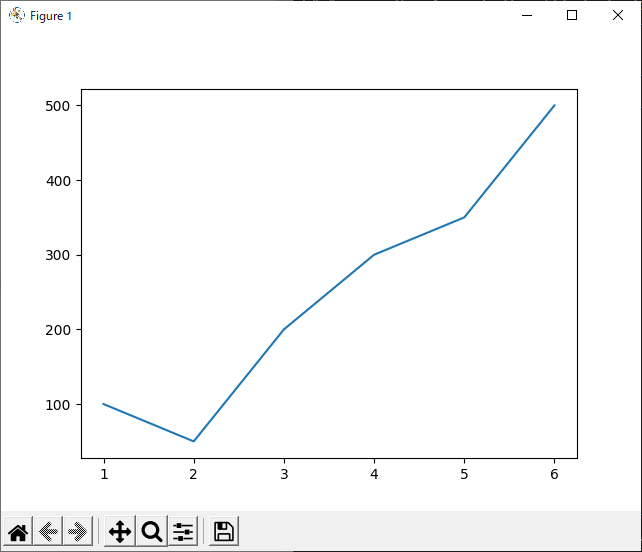
\includegraphics[width=7cm]{images/graph1.png} 

\end{legbox}
\end{pabox}

\begin{pabox}{graph-2(棒グラフ)}
6要素のデータ[200,220,240,220,260,210]の棒グラフを描画してみましょう。
基本的なグラフはx軸の値とy軸の値を指定することで簡単に表示することができます。
\begin{legbox}{class1-2.py}
\begin{listing}{1}
import matplotlib.pyplot as plt

x = [ 1, 2, 3, 4, 5, 6 ]
data = [ 200, 220, 240, 220, 260, 210 ]
label = [ '西区']
#データラベルを指定することもできる
plt.bar( x, data )
#barを使ってデータを指定します。
plt.show()
\end{listing}


実行結果\\

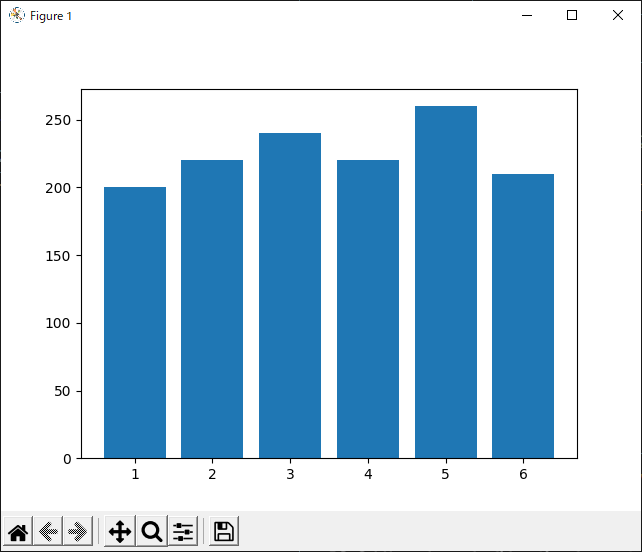
\includegraphics[width=7cm]{images/graph2.png} 

\end{legbox}
\end{pabox}


\begin{pabox}{graph-3(円グラフ)}
6要素のデータ[100,200,300,400,500,600]の円グラフを描画してみましょう。
\begin{legbox}{graph1-3.py}
\begin{listing}{1}
import matplotlib.pyplot as plt

data = [ 100, 200, 300, 400, 500, 600 ]
plt.pie( data )
#pieを使ってデータを指定します。
plt.show()
\end{listing}


実行結果\\

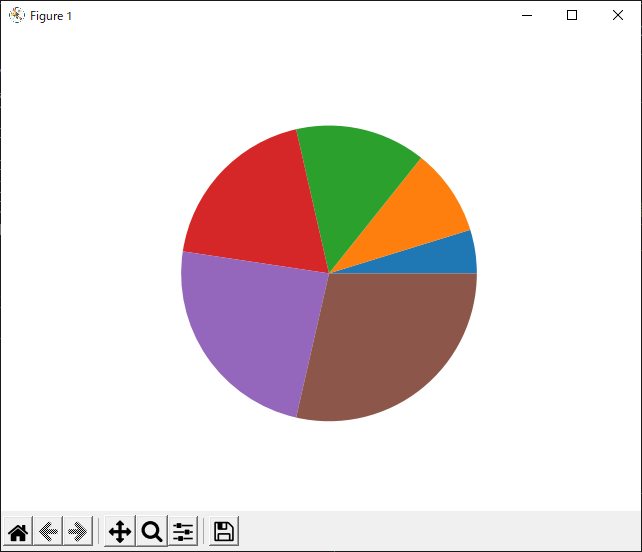
\includegraphics[width=7cm]{images/graph3.png} 

\end{legbox}
\end{pabox}

\begin{pabox}{graph-4(データラベル)}
graph-2の棒グラフのデータラベルに日本語でラベルを設定してみましょう。
\begin{legbox}{graph1-4.py}
\begin{listing}{1}
import matplotlib.pyplot as plt

#日本語フォントを設定
from matplotlib import rcParams
rcParams['font.family'] = 'sans-serif'
rcParams['font.sans-serif'] = ['Yu Gothic', 'Meirio']

x = [ 1, 2, 3, 4, 5, 6 ]
data = [ 200, 220, 240, 220, 260, 210 ]
label = [ '西区','東区','南区','北区','豊平区','手稲区']
#データラベルを指定することもできる
plt.bar( x, data ,tick_label = label)

plt.show()
\end{listing}


実行結果\\

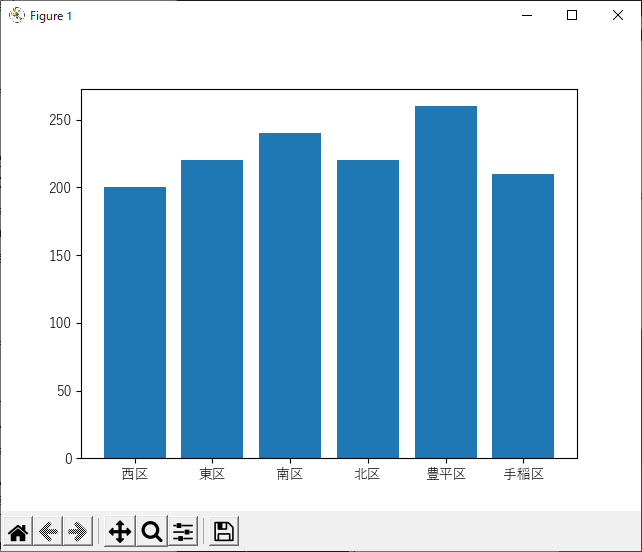
\includegraphics[width=7cm]{images/graph4.png} 

\end{legbox}
\end{pabox}


\section{numpy入門}
行列要素等の複数要素に対して効率よく処理をするためのライブラリがnumpyとなります。
\subsection{numpyの利用}

numpyの利用時にimportはasを使って「np」という別名を使うのが慣例となっています。

\begin{verbatim}
import numpy as np

\end{verbatim}


\begin{pabox}{numpy-1}
numpyを使ったデータ処理の一例を見てみましょう。
ここではリストとの違いを確認してみます。

\begin{legbox}{numpy1-1.py}
\begin{listing}{1}
import numpy as np

#listの生成
a = [ 1, 2, 3, 4, 5]
print(a)
#配列要素の生成
b = np.array([ 1, 2, 3, 4, 5])
print(b)
#listの長さが2倍
print( a * 2 )
#配列要素の中身がそれぞれ2倍
print( b * 2 )
#配列要素の要素同士が乗算される
print( b * b )
\end{listing}

実行結果\\
\begin{listing}{1}
[1, 2, 3, 4, 5]
[1 2 3 4 5]
[1, 2, 3, 4, 5, 1, 2, 3, 4, 5]
[ 2  4  6  8 10]
[ 1  4  9 16 25]
\end{listing}
\end{legbox}

\end{pabox}

\begin{pabox}{numpy-2}
numpyを使ったデータ生成の方法を見てみましょう。
ここでは関数(メソッド)を使った配列要素の生成方法を確認します。

\begin{legbox}{numpy1-2.py}
\begin{listing}{1}
import numpy as np

#rangeとよく似ていますが、整数以外も生成可能
print(np.arange(5))
print(np.arange(0, 2, 0.4))
#linspaceを使うと値を等分したリストを生成可能
print(np.linspace(0,100,5))
#10個の配列要素としての乱数を同時生成
print(np.random.rand(10))
\end{listing}

実行結果(例)\\
※乱数はそれぞれ出力される内容が異なります。\\
\begin{listing}{1}
[0 1 2 3 4]
[0.  0.4 0.8 1.2 1.6]
[  0.  25.  50.  75. 100.]
[0.61920954 0.29684569 0.94695251 0.79888711 0.77976444 0.10481961
 0.83043277 0.03716237 0.26022265 0.22519305]
\end{listing}
\end{legbox}

\end{pabox}


\begin{pabox}{numpy-3}
numpyを使った条件判定を見てみましょう。
配列要素として乱数を生成し特定の値がいくつ含まれているか数えてみましょう。

\begin{legbox}{numpy1-3.py}
\begin{listing}{1}
import numpy as np

ransu = np.random.randint(1, 4, 10)
print(ransu)
#3のところを確認する
print(ransu == 3)
#3の数を数える
print(np.count_nonzero(ransu == 3))
\end{listing}

実行結果(例)\\
※乱数はそれぞれ出力される内容が異なります。\\
\begin{listing}{1}
[2 3 1 1 1 2 2 2 3 3]
[False  True False False False False False False  True  True]
3
\end{listing}
\end{legbox}

\end{pabox}

【高等学校情報科「情報1教員研修用教材(本編)】第3章で用いられている確定モデルと確率モデルに出てくるnumpyとmatplotlibについて今まで学習した内容と合わせて確認しましょう。

\begin{pabox}{numpy-4}
参考資料「【高等学校情報科「情報1」教員研修用教材(本編)】第3章」139ページのサンプルプログラムを修正し、描画を見ながら確率モデルを確認しましょう。

\begin{legbox}{numpy1-4.py}
\begin{listing}{1}
import numpy as np # 整数をカウントするための関数呼び出し
import matplotlib.pyplot as plt # グラフプロットの呼び出し

for times in range(1,11):
    saikoro = np.random.randint(1, 6+1, 6 ** times) # サイコロを振る
    deme = [ ] # 出目の数を数える配列
    for i in range(6):
        deme.append(np.count_nonzero(saikoro==i+1)) 
  # 数を数えて配列に追加
    left = [1, 2, 3, 4, 5, 6] # グラフの左方向の値指定用
    plt.cla()
    plt.title("SAIKORO SIMULATION " + str(6 ** times) + " KAI") 
                    # グラフのタイトル
    plt.xlabel("ME") #X 軸のラベル
    plt.ylabel("KAISUU") #Y 軸のラベル
    plt.bar(left, deme, align="center") # グラフをプロット
    plt.draw() 
    plt.pause(2)
plt.show()
\end{listing}

実行結果\\

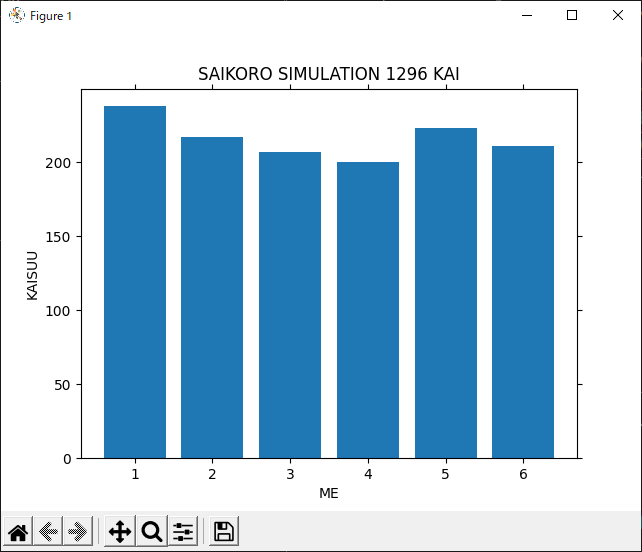
\includegraphics[width=5cm]{images/graph5.png} 

\end{legbox}


\end{pabox}

\begin{pabox}{numpy-5}
numpyとmatplotlibを使って三角関数のsinカーブを書いてみましょう。

コンピューター内部の角度は「°」ではなくradian単位を使うことが多いです。
0°から時計回り半周で円周率π(3.141592・・・・)となり、一周で2πとなるように表現される角度の単位です。

\begin{legbox}{numpy1-5.py}
\begin{listing}{1}
import numpy as np 
import matplotlib.pyplot as plt

#sinカーブの描画のための-180°~180までのradian設定
kakudo = np.linspace( -np.pi, np.pi, 361)
x = np.linspace(-180,180,361)
plt.plot(x, np.sin(kakudo))
plt.show()
\end{listing}

実行結果\\

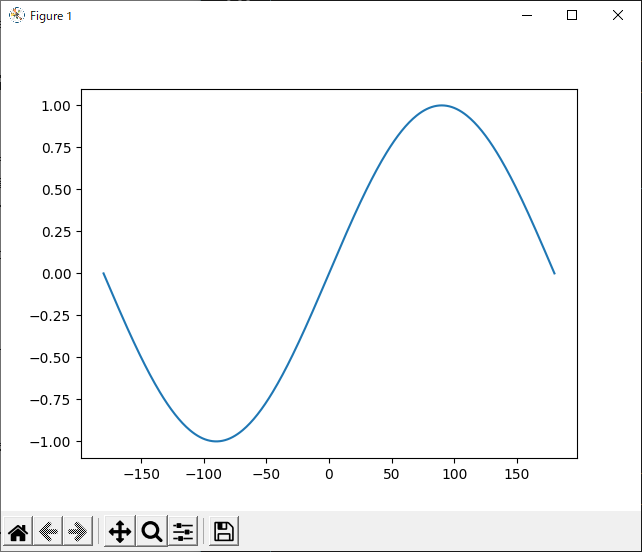
\includegraphics[width=6cm]{images/graph6.png} 

\end{legbox}


\end{pabox}
このような数値計算を効率よく行うためのライブラリがnumpyライブラリとなります。

\section{WebAPIの利用}
ここではWebAPIによるJSONデータの取得を行い、グラフで視覚化してみます。

WebAPIを使ったJSONデータの取得方法とデータ構造は次の通りとなります。






